% VLDB-Template enhances the ACM master template, acmart.cls v2.19 (2026/06/27):
% https://www.acm.org/publications/proceedings-template
% The ACM Latex guide provides further information about the ACM template
%
% This bundle pins acmart.cls v2.19 (rather than relying on whatever version
% ships with an author's local TeX install or Overleaf project) to guarantee
% consistent formatting across all PVLDB submissions.

\documentclass[sigconf, nonacm]{acmart}
\usepackage{multirow}

%%% do not modify the following VLDB block %%
%%% VLDB block start %%%
\usepackage{pvldb}% VLDB/PVLDB formatting overrides, see pvldb.sty for details.
                      % Do not remove -- required for consistent proceedings
                      % formatting across all VLDB submissions.
%%% VLDB block end %%%

%% The following must be set for each paper (values below are placeholders).
%% Everything else (volume/issue/year defaults, the PVLDB Reference Format
%% block, license footer, and Artifact Availability block) is handled by
%% pvldb.sty -- see that file if you need to change shared defaults.
\renewcommand\vldbdoi{XX.XX/XXX.XX}
\renewcommand\vldbpages{XXX-XXX}
% VLDB is single-blind (see submission guidelines): the real, public code/data
% repository goes here, not an anonymized mirror. Fill in once the repo is
% public and contains the code, run scripts, and instructions to reproduce
% every number in the paper.
\renewcommand\vldbavailabilityurl{https://github.com/samjhana-bhusal/sql-indexing-with-rmi}

\begin{document}
%% NOTE: append the category tag to the title if submitting as a
%% non-Regular-Research paper (both in this PDF and in the CMT submission
%% title). See "Category tag" note in the accompanying steps.
\title{Evaluating the Memory--Compute Trade-offs of Learned Index Structures with LSM-style Dynamic Write Buffers and Drift-Triggered Maintenance [Experiment, Analysis \& Benchmark]}

%% VLDB is single-blind: real names and affiliations are required on the
%% first page. Replace the EMAIL placeholders below with the actual
%% addresses -- left as placeholders here rather than guessed.
\author{Samjhana Bhusal}
\affiliation{%
  \institution{Cedargate Technologies}
  \city{Kathmandu}
  \country{Nepal}
}
\affiliation{%
  \institution{Kathmandu University}
  \city{Dhulikhel}
  \country{Nepal}
}
\email{SAMJHANA_PERSONAL_EMAIL}


\begin{abstract}
Traditional database indexes, primarily B+Trees, suffer from significant latency overheads and high cache miss rates due to pointer-chasing in memory-bound architectures. The emerging paradigm of Learned Indexes addresses this by treating the indexing problem as a Cumulative Distribution Function (CDF) prediction task, replacing tree traversal with numerical model execution. However, static learned indexes like the Recursive Model Index (RMI) do not natively support dynamic insertions without expensive retraining. 

In this work, we present a hybrid C++/Python execution pipeline comparing a degree-optimized ($B=64$) C++ B+Tree against a two-stage CPU/GPU RMI. To address the dynamic update bottleneck, we implement an LSM-style Delta Buffer (Write-Ahead Store) integrated with our RMI. Our experiments show that the RMI achieves a 99.97\% memory footprint compression (117.9~KB vs. 334.7~MB) and significantly lowers latency compared to the B+Tree under continuous distributions. We evaluate RMI sensitivity across uniform, log-normal, and clustered key distributions, including a drifting workload where the key distribution shifts over time. We demonstrate how our dynamic write buffer maintains low-latency lookups ($<0.11\,\mu$s) while supporting real-time inserts. Using a merge-based workload in which the delta buffer is periodically compacted into the sorted array (so that an unmaintained model genuinely decays), we show that a never-retrained learned index is not viable under drift: its lookups fall back to a full search $99.8\%$ of the time, making it both the least accurate \textit{and} the slowest policy. We then introduce a \textit{drift-triggered adaptive retraining} mechanism that monitors per-segment prediction error and key distribution and selectively refits only degraded Stage~2 leaf models, reaching $96\%$ of full periodic-retraining throughput while refitting only $24.6\%$ as many segments.
\end{abstract}

\maketitle

%%% do not modify the following VLDB block %%
%%% VLDB block start %%%
\vldbtopmatter
%%% VLDB block end %%%

\section{Introduction}
Modern computer systems are increasingly constrained by the ``Memory Wall'': the growing performance gap between fast CPU core executions and slow DRAM data fetches~\cite{wulf1995hitting, hennessy2011computer}. In relational database storage engines, index lookups represent a critical bottleneck. The ubiquitous B+Tree index~\cite{comer1979ubiquitous} navigates sorted datasets by traversing child node pointers, resulting in multiple random memory accesses. Because these heap-allocated nodes are rarely aligned in cache lines, B+Tree lookups trigger significant L1/L2 data cache misses and cause CPU pipeline stalls.

To resolve this memory-bound bottleneck, Kraska et al.~\cite{kraska2018case} proposed replacing traditional index trees with Machine Learning (ML) regression models that learn the Cumulative Distribution Function (CDF) of the keys. By utilizing a key as a model input, the learned index directly predicts its physical offset in a sorted data array:
\begin{equation}
    \text{Predicted\_Position} = F(x) \times N
\end{equation}
where $F(x) \in [0,1]$ is the learned CDF of the dataset, and $N$ is the dataset size. Because the prediction has an associated error bound $\epsilon$, the exact index is located by running a local binary search within the bounded window:
\begin{equation}
    [\text{Predicted\_Position} - \epsilon, \text{Predicted\_Position} + \epsilon]
\end{equation}
This approach shifts the workload from memory fetches (pointer-chasing) to arithmetic pipeline calculations (neuron evaluations), improving cache utilization and throughput. 

Despite these benefits, static learned indexes (such as the standard Recursive Model Index) suffer from the \textit{Dynamic Update Problem}: inserting new keys alters the dataset's CDF, requiring full model retraining. In this paper, we address this issue by proposing, implementing, and evaluating a dynamic read-write hybrid index that merges an RMI with an LSM-style Delta Buffer write store.

\medskip
\noindent\textbf{Contributions.} This paper makes the following contributions:
\begin{itemize}
    \item We characterize the memory--compute trade-off of a two-stage RMI against a degree-optimized B+Tree across uniform, log-normal, and clustered distributions, quantifying both the $99.97\%$ memory reduction and the distributions where the learned model degrades (Section~4).
    \item We show that once a delta buffer is periodically \emph{merged} into the sorted array, an unmaintained learned index decays catastrophically (falling back to a full search on $99.8\%$ of lookups), making the cost of skipping maintenance directly measurable rather than asserted (Section~5).
    \item We introduce a drift-triggered adaptive retraining policy that combines a per-segment prediction-error monitor with a two-sample Kolmogorov--Smirnov test, and show it recovers $96\%$ of full periodic-retraining throughput while refitting only $24.6\%$ as many segments, an intermediate point on a cost--quality frontier, not a strict domination (Section~5).
    \item We benchmark against the ALEX and LIPP updatable learned indexes and validate on the real-world SOSD datasets, and report an ablation showing that GPU batching does not beat a single CPU core for RMI lookups until impractically large batch sizes (Sections~4 and~6).
\end{itemize}

\section{System Architecture \& Design}
Our architecture consists of three core components: the baseline B+Tree, the hybrid two-stage RMI, and the dynamic LSM-style write buffer.

\subsection{Degree-Optimized B+Tree Baseline}
We implemented a self-contained, header-only B+Tree in C++ (Degree $B=64$) optimized for cache-line alignment. The leaf nodes store sorted key-value pairs representing raw data keys and their array positions, while internal nodes route lookup queries. We equipped the tree with a recursive memory allocation tracker to accurately capture heap capacity overhead (such as vector pre-allocations), enabling an honest comparison against learned index parameter sizes.

\subsection{Recursive Model Index (RMI) Pipeline}
Our RMI uses a two-stage hybrid layout designed in Python (using PyTorch) and compiled into optimized C++:
\begin{enumerate}
    \item \textbf{Stage 1 (Root NN)}: A feed-forward neural network with 32 hidden units and a ReLU activation. The input is a min-max scaled key:
    \begin{equation}
        x_{\text{scaled}} = \frac{Key - Min\_Key}{Max\_Key - Min\_Key}
    \end{equation}
    The network predicts a normalized target position $y \in [0,1]$.
    \item \textbf{Stage 2 (Leaf Splines)}: The predicted index $y$ selects one of $M$ independent linear models:
    \begin{equation}
        idx_{\text{leaf}} = \text{clamp}(\lfloor y \times M \rfloor, 0, M-1)
    \end{equation}
    Each leaf model $i$ stores an Ordinary Least Squares (OLS) slope $m_i$ and intercept $c_i$, fitted during training on the raw key space.
    \item \textbf{Search Bounds Calculation}: For each leaf bucket, we compute the maximum absolute error window:
    \begin{equation}
        \epsilon_i = \text{int}\left(\lceil \max_{x \in \text{Leaf}_i} | (m_i \cdot x + c_i) - \text{True\_Pos} | \rceil\right)
    \end{equation}
    We store the $\epsilon_i$ values as integers. During lookup, we run a standard local binary search within the bounded window in C++.
\end{enumerate}

\subsection{LSM-Style Delta Buffer}
To support dynamic insertions, we integrate a dynamic write store (a Red-Black Tree in C++ using \texttt{std::map}) with the RMI. When a write query is received, the key-value pair is inserted directly into the dynamic Delta Buffer, avoiding RMI retraining. When a read query occurs, the index executes a two-step lookup:
\begin{enumerate}
    \item Search the Delta Buffer. If the key exists, return the value immediately ($O(\log K)$ latency, where $K$ is the buffer size).
    \item If missing, evaluate the Stage 1 Root NN and Stage 2 linear spline to locate the search window in the static array, executing the bounded binary search.
\end{enumerate}

\begin{table*}[t]
\centering
\caption{Comprehensive Performance Metrics: B+Tree vs. RMI across Parameter Space ($M$). \textit{Protocol note:} this sweep was collected under the earlier single-run protocol without inter-trial cache flushing, so its absolute throughputs run optimistically high relative to Tables~\ref{tab:baselines} and~\ref{tab:sosd} (e.g.\ lognormal $M{=}5000$ reports $14.91$ MQPS here vs.\ $11.07 \pm 1.21$ MQPS under the 5-trial cache-flushed protocol). The \textit{relative} ordering across $M$ and across distributions is unaffected, which is what this table is used to establish.}
\label{tab:sweep_results}
\setlength{\tabcolsep}{4.5pt}
\begin{tabular}{llrrrr}
\toprule
\textbf{Distribution} & \textbf{Configuration} & \textbf{Memory} & \textbf{Avg Latency} & \textbf{Throughput} & \textbf{Max Search Error} \\
\midrule
\textbf{UNIFORM} & B+Tree Baseline & 336.84 MB & 0.2215 $\mu$s & 24.01 MQPS & -- \\
                 & RMI ($M=100$) & 3.13 KB & 0.0416 $\mu$s & 24.01 MQPS & 1.0 \\
                 & RMI ($M=1000$) & 24.23 KB & 0.0363 $\mu$s & 27.58 MQPS & 1.0 \\
                 & RMI ($M=10000$) & 235.16 KB & 0.0367 $\mu$s & 27.25 MQPS & 1.0 \\
\midrule
\textbf{LOGNORMAL} & B+Tree Baseline & 334.72 MB & 0.2115 $\mu$s & 4.74 MQPS & -- \\
                   & RMI ($M=100$) & 3.13 KB & 0.1100 $\mu$s & 9.08 MQPS & 481.0 \\
                   & RMI ($M=1000$) & 24.23 KB & 0.0893 $\mu$s & 11.19 MQPS & 193.0 \\
                   & RMI ($M=5000$) & 117.98 KB & 0.0670 $\mu$s & 14.91 MQPS & 109.0 \\
\midrule
\textbf{CLUSTERED} & B+Tree Baseline & 336.75 MB & 0.2164 $\mu$s & 4.51 MQPS & -- \\
                   & RMI ($M=100$) & 3.13 KB & 0.5409 $\mu$s & 1.84 MQPS & 1,936,055.0 \\
                   & RMI ($M=1000$) & 24.23 KB & 0.5045 $\mu$s & 1.98 MQPS & 996,834.0 \\
\bottomrule
\end{tabular}
\end{table*}

\section{Hardware Architecture Analysis}
Traditional B+Trees represent a classic memory-bound bottleneck:
\begin{equation}
    \text{Memory Stalls} = \text{Misses} \times \text{Miss Penalty}
\end{equation}
Traversing a B+Tree of height $H$ requires chasing $H$ pointers. If the nodes are not in CPU cache, each redirection results in a main-memory fetch ($\approx 50$--$100\,$ns delay), causing the CPU instruction execution pipelines to stall. This leads to a low Instructions Per Cycle (IPC) rate.

Conversely, our RMI fits completely inside the CPU cache. The total parameter space for $M=5000$ leaf models is only $117.97$ KB. This tiny profile fits within standard L2 caches. Consequently, the CPU executes Stage~1 matrix multiplications and Stage~2 linear spline interpolation using cached registers, shifting execution to compute pipelines and maximizing the CPU's IPC.

\section{Experimental Methodology \& Evaluation}
Our benchmarks evaluate the indexing structures under three key aspects: trade-off frontiers, distribution sensitivity, and write-buffering scalability. All tests were executed on an Apple Silicon host architecture featuring Unified Memory.

\subsection{Parameter Sweep Analysis}
Table~\ref{tab:sweep_results} shows the empirical results of our comprehensive parameter sweep. Under a \textbf{Uniform} distribution, the RMI exhibits an ideal linear structure. The maximum absolute search error is clamped at exactly $1.0$ across all values of $M$. Consequently, the local search window requires at most a single local step, enabling the RMI to outpace the B+Tree's lookup latency by over \textbf{6$\times$} ($0.036\,\mu$s vs $0.221\,\mu$s) while using $99.99\%$ less index memory.

For the skewed \textbf{Log-Normal} distribution, expanding the leaf allocation space from $M=100$ to $M=5000$ divides the maximum prediction error from $481.0$ to $109.0$. This smaller error tightens the bounded binary search space, improving average CPU lookup latency from $0.110\,\mu$s to $0.067\,\mu$s, outperforming the B+Tree baseline ($0.210\,\mu$s) by a factor of 3.14$\times$.

\begin{figure}[t]
    \centering
    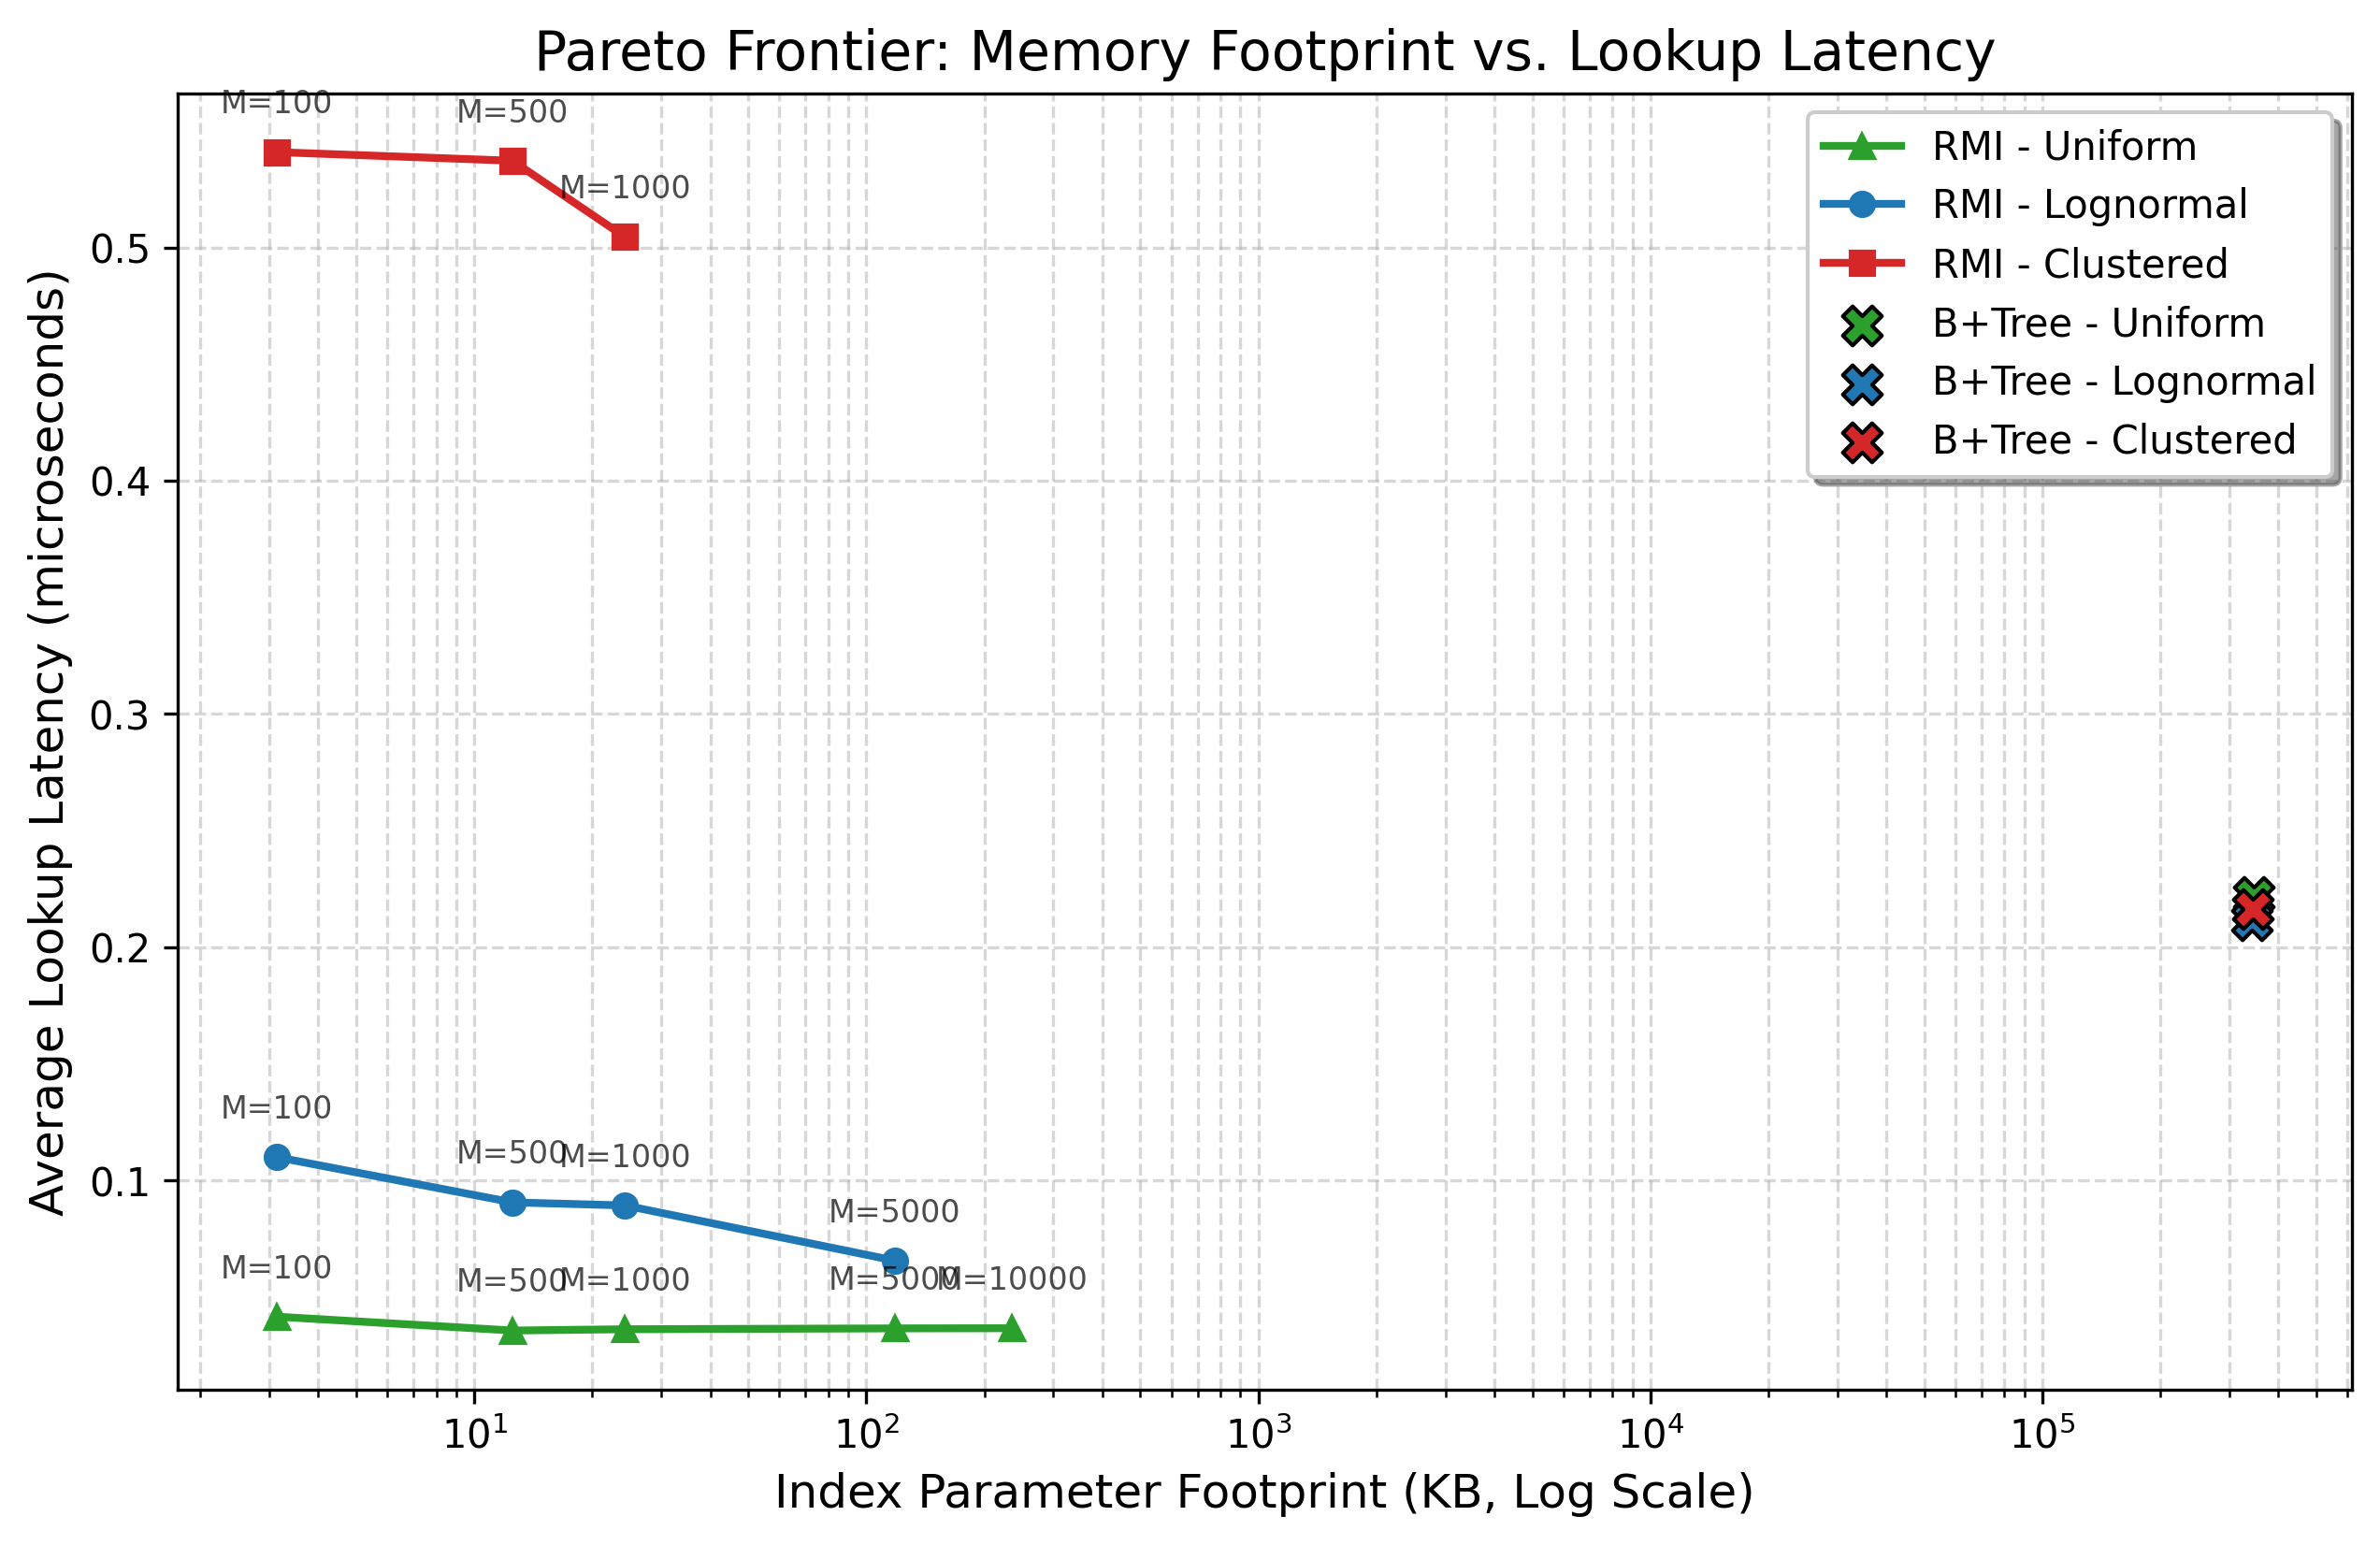
\includegraphics[width=\linewidth]{pareto_frontier.png}
    \caption{Pareto Frontier analysis tracking Index Parameter Memory Footprint vs. Lookup Latency under varying key distributions.}
    \Description{Scatter plot of lookup latency versus memory footprint for the RMI at several leaf counts and for the B+Tree baseline, across uniform, log-normal, and clustered key distributions.}
    \label{fig:pareto}
\end{figure}

\subsection{Distribution Breakdown and Boundary Fragility}
As shown in Fig.~\ref{fig:pareto}, the performance of the RMI degrades heavily when exposed to an adversarial \textbf{Clustered} distribution. Because the dataset features dense clumps separated by massive empty data gaps, the Stage 1 root network misroutes keys across boundaries. This causes the OLS models inside the leaves to span wide empty ranges, inflating the maximum search error to $996,834$ elements for $M=1000$.

When the search window expands to include nearly $10\%$ of the entire index space, the local bounded lookup reverts into a heavy un-cached binary search over megabytes of main memory. This structural fragility slows RMI latency to $0.504\,\mu$s, making it more than twice as slow as the distribution-oblivious B+Tree ($0.216\,\mu$s). At configurations of $M \ge 5000$, this mismatch causes integer boundary overflows or underflows in C++ pointer tracking loops unless explicit index clamping guardrails are applied.

\subsection{Dynamic Write Buffering Scalability}
To validate real-time updates, we tested an evaluation pipeline running $10,000$ sequential dynamic insertions followed by lookups under varying delta-buffer configurations on the log-normal dataset. 

The LSM-style write path achieved an outstanding average insertion speed of \textbf{0.0230~$\mu$s/write}. However, as the un-indexed data accumulation within the Red-Black tree grows, lookup latencies degrade due to sequential verification lookups across multiple data blocks. At a buffer size of $0$, lookup latency matches the base RMI speed of $0.058\,\mu$s. As the buffer scales to $1,000$ and $10,000$ keys, lookup latency increases to $0.078\,\mu$s and $0.105\,\mu$s respectively, reflecting a clear memory-compute performance trade-off.

\begin{table}[h]
\centering
\caption{Dynamic Read-Write Performance (Lognormal)}
\label{tab:delta_buffer}
\begin{tabular}{rrr}
\toprule
\textbf{\shortstack{Buffer\\Size}} & \textbf{\shortstack{Write Latency\\($\mu$s)}} & \textbf{\shortstack{Read Latency\\($\mu$s)}} \\
\midrule
0     & 0.0230 & 0.0589 \\
100   & 0.0230 & 0.0647 \\
1000  & 0.0230 & 0.0784 \\
5000  & 0.0230 & 0.0991 \\
10000 & 0.0230 & 0.1051 \\
\bottomrule
\end{tabular}
\end{table}

\subsection{The Cost of GPU Dispatch: Batch Size Sensitivity}
We ported the multi-stage RMI lookup to Apple Silicon's MPS GPU framework and swept batch sizes from 1 to 65{,}536 over 100{,}000 queries, measuring throughput and GPU memory allocation at each point (5-run mean$\pm$stddev). This is an \textit{ablation} designed to answer: how large must a batch be before GPU dispatch amortizes against the tiny per-query compute of an RMI lookup?

\begin{figure}[h]
    \centering
    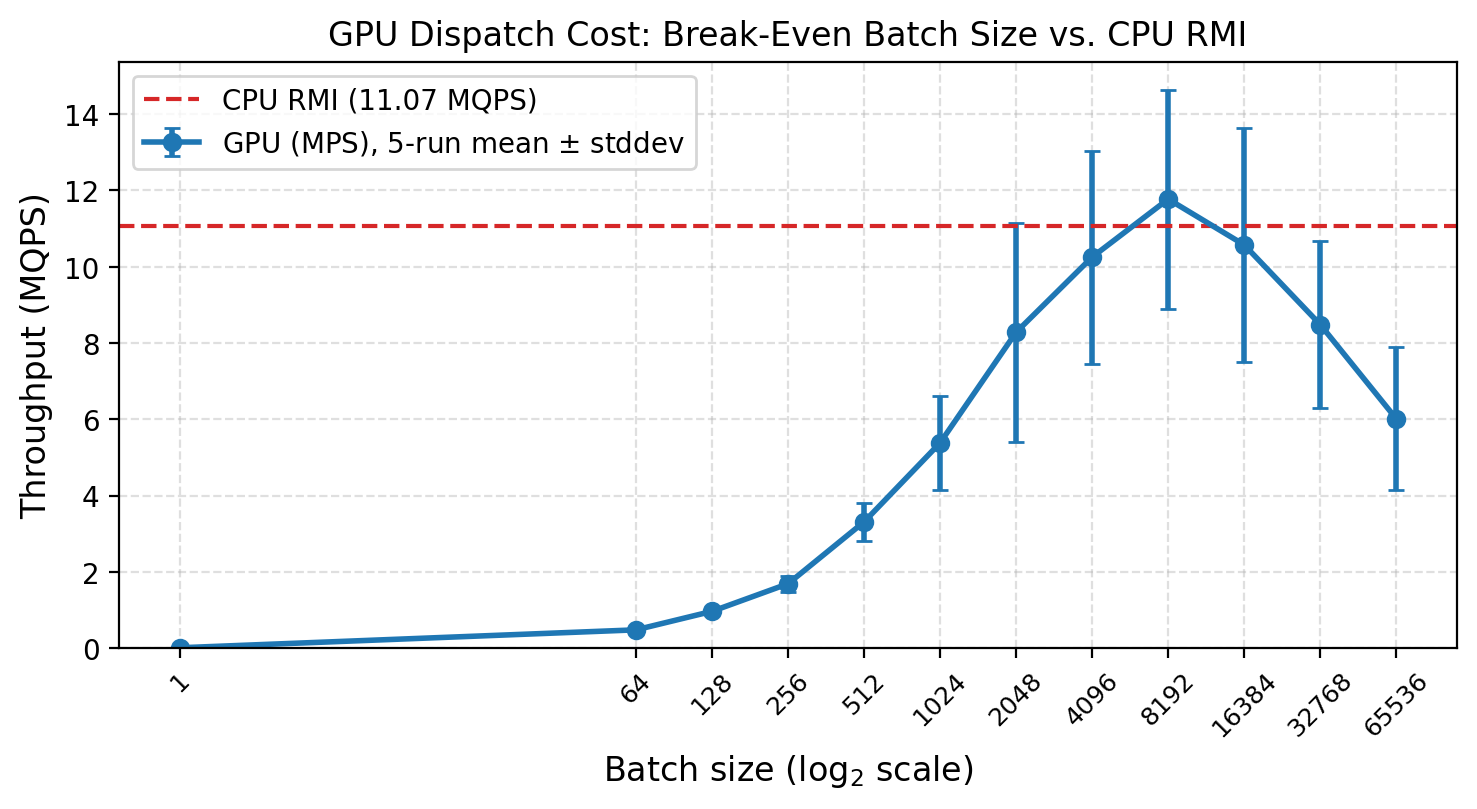
\includegraphics[width=\linewidth]{gpu_throughput.png}
    \caption{GPU throughput across a log$_2$ sweep of batch sizes (5-run mean, error bars $\pm 1$ stddev). The dashed line marks CPU RMI throughput (11.07 MQPS). Throughput rises to batch $8192$, where it reaches parity with the CPU, then declines. GPU memory allocation was essentially constant across the sweep ($76.6$--$78.3$~MB) and is omitted.}
    \Description{Line plot of GPU throughput in millions of queries per second against batch size on a log base two scale, with error bars, compared against a horizontal reference line for CPU RMI throughput.}
    \label{fig:gpu_throughput}
\end{figure}

\begin{table}[h]
\centering
\caption{GPU throughput vs.\ batch size (MPS, 5-run mean$\pm$stddev). CPU RMI baseline is $11.07 \pm 1.21$ MQPS.}
\label{tab:gpu_sweep}
\begin{tabular}{rrrr}
\toprule
\textbf{Batch} & \textbf{MQPS} & \textbf{Batch} & \textbf{MQPS} \\
\midrule
1    & $0.008 \pm 0.000$ & 2048  & $8.28 \pm 2.87$ \\
64   & $0.478 \pm 0.036$ & 4096  & $10.25 \pm 2.79$ \\
128  & $0.963 \pm 0.027$ & \textbf{8192}  & $\mathbf{11.77 \pm 2.87}$ \\
256  & $1.686 \pm 0.203$ & 16384 & $10.57 \pm 3.07$ \\
512  & $3.308 \pm 0.490$ & 32768 & $8.48 \pm 2.19$ \\
1024 & $5.380 \pm 1.234$ & 65536 & $6.01 \pm 1.87$ \\
\bottomrule
\end{tabular}
\end{table}

The answer is: very large. At batch=1, per-dispatch overhead throttles throughput to $0.008$~MQPS, roughly $1400\times$ slower than the CPU, since every lookup pays a full kernel launch to do $\sim$100 FLOPs of work. Throughput then rises monotonically with batch size, peaking at \textbf{$11.77 \pm 2.87$~MQPS at batch=8192}. At that point the GPU is \textit{statistically indistinguishable} from the CPU RMI ($11.07 \pm 1.21$~MQPS; the intervals overlap substantially). Beyond 8192 throughput declines again: the loop iteration count falls into single digits, so per-dispatch overhead is amortized over fewer and fewer launches and measurement variance grows.

The practical conclusion is not that the GPU is incapable, but that the \textit{break-even batch size is prohibitive}. Reaching mere parity with one CPU core requires accumulating $8{,}192$ independent lookups per dispatch, a level of query concurrency that point-lookup workloads in a storage engine rarely exhibit, and which would impose latency cost on every query while the batch fills. Each RMI lookup is $\sim$100 FLOPs (32-neuron hidden layer $+$ one linear spline), far too little to amortize kernel launch latency individually. Extracting a genuine \textit{speedup} rather than parity would require fusing the multi-stage lookup into a single kernel and pipelining CPU$\to$GPU transfers with double-buffering. The honest result is therefore a cost-benefit one: naive GPU batching buys no throughput over a single CPU core until batch sizes become impractically large.

\section{Adaptive Retraining for Learned Indexes}

The LSM-style delta buffer (Section~2.3) defers the cost of dynamic inserts, but deferral is not free forever: a delta buffer must eventually be \textit{merged} back into the sorted base array, or lookups on buffered keys degrade to an $O(\log K)$ secondary-structure probe and the buffer's memory grows without bound. The moment we merge, every key's rank (its position in the sorted array) shifts, and the Stage~2 models, which predict exactly that rank, go stale. Their error bounds are now violated: a bounded search over $[\hat{p}-\epsilon,\hat{p}+\epsilon]$ no longer contains the key, forcing a full-array fallback that is correct but $O(\log N)$-wide. This is the concrete mechanism by which an unmaintained learned index decays under drift.

Periodic full retraining, refitting all $M$ Stage~2 leaf models after every merge, eliminates the decay but is wasteful when only a minority of segments actually drifted. We introduce a \textit{drift-triggered localized retraining} mechanism that monitors per-segment prediction error and key distribution, and selectively refits only the degraded segments after each merge.

\subsection{Drift Monitor Design}

Our drift monitor tracks two complementary signals per segment~$i$:

\begin{enumerate}
    \item \textbf{Prediction error ratio.} A running mean of absolute prediction error on recent lookups. When $\bar{e}_i > \alpha \cdot \epsilon_{\max,i}$ (where $\epsilon_{\max,i}$ is the training-time max error for segment~$i$ and $\alpha = 1.5$ by default), segment~$i$ is flagged for retraining.
    \item \textbf{Two-sample Kolmogorov-Smirnov test.} After each batch of inserts, buffer keys mapped to segment~$i$ are compared against the original training keys using a KS test ($p < 0.01$). This catches distributional shift proactively, before prediction error has grown.
\end{enumerate}

When a segment is flagged, its Stage~2 OLS model (slope, intercept, max-error) is refit against the keys the router now assigns to it in the merged array. Cost per segment: one pass over $\sim N/M$ keys ($\sim$sub-millisecond for $N=10^6$, $M=500$).

\subsection{Evaluation: Adaptive vs.\ Periodic vs.\ Never-Retrain}

\noindent\textbf{Workload.} We evaluate three maintenance policies on a \textit{drifting} insert workload: $N=10^6$ base keys ($M=500$ segments), then $200{,}000$ inserts delivered in $20$ windows of $10{,}000$. The first half of the inserts fall within the original key range; the second half are shifted beyond $\max(\text{key})$, a genuine covariate shift the Stage~1 router never saw. After each window the delta buffer is merged into the sorted array, and the policy decides what to refit: \textbf{never} (nothing), \textbf{periodic} (all $M$ segments), or \textbf{adaptive} (only drift-flagged segments). We report, per window, read throughput, p99 lookup latency, and \textit{bound-miss rate}: the fraction of lookups whose model-predicted window failed and fell back to a full search, the direct, measured signal of model staleness.

\begin{table*}[t]
\centering
\caption{Maintenance-policy comparison under a drifting merge workload ($N{=}10^6$, $M{=}500$; $200$k inserts over $20$ merges; 5-run mean$\pm$stddev). Metrics are averaged over the run. ``Segs retrained'' is the total across all $20$ merges.}
\label{tab:adaptive}
\begin{tabular}{lrrrr}
\toprule
\textbf{Policy} & \textbf{MQPS} & \textbf{p99 ($\mu$s)} & \textbf{Bound-miss \%} & \textbf{Segs retrained} \\
\midrule
Never retrain    & $7.09 \pm 0.25$ & $0.499 \pm 0.018$ & $99.76 \pm 0.01$ & $0$ \\
Periodic retrain & $\mathbf{9.09 \pm 0.12}$ & $\mathbf{0.368 \pm 0.017}$ & $\mathbf{0.00 \pm 0.00}$ & $10{,}000$ \\
Adaptive retrain & $8.73 \pm 0.39$ & $0.396 \pm 0.035$ & $27.56 \pm 1.45$ & $2{,}455 \pm 5$ \\
\bottomrule
\end{tabular}
\end{table*}

\noindent\textbf{Maintenance is not optional.} The headline result is the \textbf{never}-retrain row: under drift its bound-miss rate is $99.76\%$, essentially \textit{every} lookup falls back to a full-array search because the stale Stage~2 bounds no longer contain the shifted keys. Crucially, never-retrain is not merely inaccurate, it is also the \textit{slowest} policy ($7.09$ vs.\ $9.09$ MQPS): the fallbacks it incurs cost more than the maintenance it avoids. A static learned index is not a viable design once the data moves. This is the point the earlier version of this work asserted but did not measure; the merge-based evaluation now demonstrates it directly.

\noindent\textbf{Selective vs.\ full retraining.} Periodic retraining is the quality ceiling: $0\%$ bound-miss and the best throughput, at the cost of refitting all $10{,}000$ segment-instances over the run. Adaptive retraining reaches $96\%$ of periodic's throughput ($8.73$ vs.\ $9.09$ MQPS) while refitting only $24.6\%$ as many segments ($2{,}455$ vs.\ $10{,}000$). It does not, however, match periodic's correctness: its $27.6\%$ average bound-miss reflects a one-window detection \textit{lag}, visible as the oscillation in Fig.~\ref{fig:adaptive} (left); each merge drifts fresh segments that adaptive only repairs on the following window. Adaptive thus occupies an intermediate point on a cost--quality trade-off, not a strict domination of periodic.

\noindent\textbf{On tuning.} The error-ratio threshold $\alpha$ turns out to be a weak cost lever: sweeping $\alpha \in [0.5, 10]$ moved total segments retrained only from $2{,}559$ to $2{,}122$, because the KS distributional trigger (independent of $\alpha$) accounts for most retrains under a genuine covariate shift. The effective knob is the merge/check interval, not $\alpha$, a point we return to in future work.

\begin{figure*}[t]
\centering
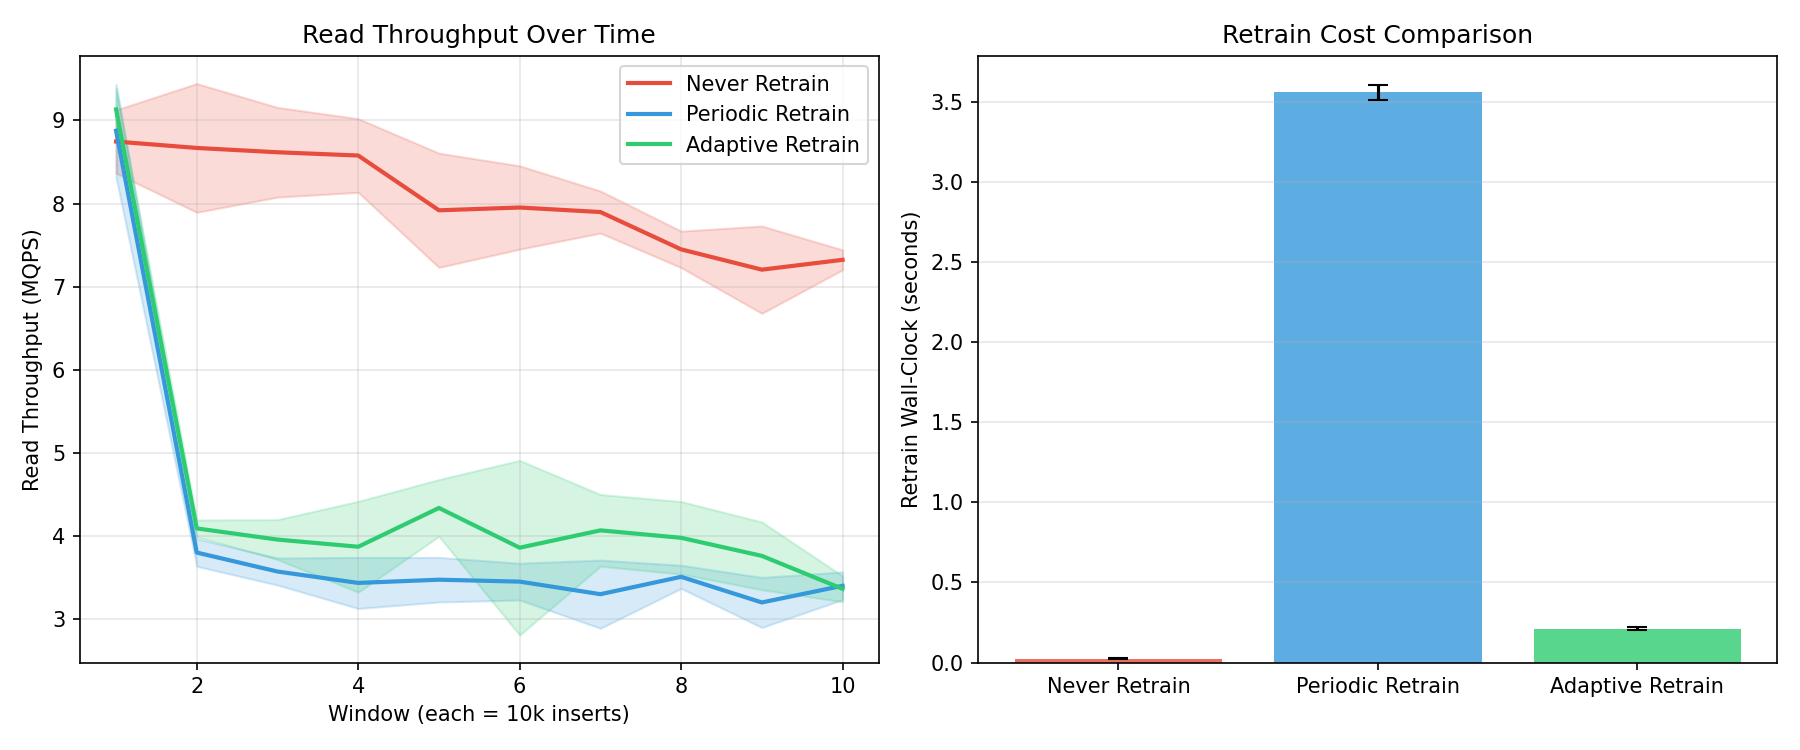
\includegraphics[width=\textwidth]{adaptive_vs_periodic.png}
\caption{Maintenance policies under a drifting merge workload (5-trial mean, shaded $\pm 1$ stddev). \textbf{Left:} bound-miss rate over time: never-retrain is pinned near $100\%$; adaptive oscillates as it repairs drift one window behind; periodic stays at zero. \textbf{Center:} p99 lookup latency. \textbf{Right:} total maintenance cost (segments retrained); adaptive is $24.6\%$ of periodic.}
    \Description{Three-panel plot comparing never-retrain, periodic-retrain, and adaptive-retrain maintenance policies over time: bound-miss rate, p99 lookup latency, and total segments retrained.}
\label{fig:adaptive}
\end{figure*}

\section{Baseline Comparison: ALEX and LIPP}

To position our RMI against the state of the art in updatable learned indexes, we benchmark two external baselines on the same synthetic and SOSD~\cite{marcus2020benchmarking} datasets:

\begin{itemize}
    \item \textbf{ALEX}~\cite{ding2020alex}: Microsoft's adaptive learned index. ALEX maintains a gapped array of data nodes with per-node linear models, dynamically splitting and retraining nodes on insert. We use the official C++ header-only implementation with ARM compatibility patches for Apple Silicon.
    \item \textbf{LIPP}~\cite{wu2021lipp}: an updatable learned index whose models predict \emph{precise} positions, eliminating the last-mile search, and which absorbs updates by splitting nodes. We use the reference C++ implementation.
\end{itemize}

Both baselines are bulk-loaded with the same sorted key-value pairs and evaluated with the same 100{,}000-query random lookup workload (5-run mean$\pm$stddev, inter-trial cache flush). Table~\ref{tab:baselines} shows the results on the lognormal synthetic dataset ($N{=}10$M).

\begin{table*}[t]
\centering
\caption{Read-only lookup comparison on lognormal $N{=}10$M (5-run mean$\pm$stddev, inter-trial cache flush).}
\label{tab:baselines}
\begin{tabular}{lrrr}
\toprule
\textbf{Index} & \textbf{Memory} & \textbf{Throughput (MQPS)} & \textbf{Latency ($\mu$s)} \\
\midrule
B+Tree ($B{=}64$) & 334.72 MB & $4.00 \pm 0.72$ & $0.259$ \\
RMI ($M{=}5000$)   & \textbf{117.98 KB} & $11.07 \pm 1.21$ & $0.091$ \\
ALEX~\cite{ding2020alex}   & 218.31 MB & $14.98 \pm 4.51$ & $0.080$ \\
LIPP~\cite{wu2021lipp}     & 710.07 MB & $\mathbf{22.74 \pm 5.80}$ & $\mathbf{0.049}$ \\
\bottomrule
\end{tabular}
\end{table*}

\medskip

The comparison highlights the trade-off each design makes. ALEX and LIPP are \textit{natively updatable}: they absorb inserts without an external buffer or retraining step, at the cost of higher per-node metadata overhead and more complex internal restructuring. ALEX maintains gapped arrays with per-node linear models that split and retrain dynamically on insert; LIPP stores precise positions so lookups need no local search, at the cost of storing that structure explicitly; at $710$~MB it consumes the most memory of all tested indexes. Our RMI, by contrast, uses a decoupled delta buffer and drift-triggered localized retraining (Section~5). While LIPP and ALEX achieve higher raw throughput, the RMI's $118$~KB footprint is \textit{three orders of magnitude smaller} than any competitor, small enough to fit entirely in L2 cache, making it the preferred choice when memory is constrained or when the working set must coexist with other in-memory structures.

\subsection{Validation on Real-World Data (SOSD)}
Synthetic distributions are smooth and parametric by construction, which flatters learned indexes. To test whether our conclusions survive contact with real key distributions, we repeat the identical evaluation on two SOSD~\cite{marcus2020benchmarking} datasets: \textbf{books} (Amazon book sale popularity, $11.42$M unique keys after deduplication) and \textbf{wiki\_ts} (Wikipedia edit timestamps, $3.37$M unique keys). Table~\ref{tab:sosd} reports the results.

\begin{table*}[t]
\centering
\caption{Lookup performance on SOSD real-world datasets (5-run mean$\pm$stddev, inter-trial cache flush).}
\label{tab:sosd}
\begin{tabular}{llrrr}
\toprule
\textbf{Dataset} & \textbf{Index} & \textbf{Memory} & \textbf{Throughput (MQPS)} & \textbf{Latency ($\mu$s)} \\
\midrule
\multirow{4}{*}{\textbf{books}}
 & B+Tree & 384.66 MB & $4.00 \pm 0.65$ & $0.259$ \\
 & RMI    & \textbf{117.98 KB} & $10.42 \pm 1.23$ & $0.097$ \\
 & ALEX   & 250.88 MB & $\mathbf{11.08 \pm 1.78}$ & $\mathbf{0.093}$ \\
 & LIPP   & \multicolumn{3}{c}{n/a (see note)} \\
\midrule
\multirow{4}{*}{\textbf{wiki\_ts}}
 & B+Tree & 113.35 MB & $5.49 \pm 0.39$ & $0.183$ \\
 & RMI    & \textbf{117.98 KB} & $14.08 \pm 0.59$ & $0.071$ \\
 & ALEX   & 78.07 MB  & $15.32 \pm 0.84$ & $0.065$ \\
 & LIPP   & 331.79 MB & $\mathbf{18.46 \pm 1.89}$ & $\mathbf{0.055}$ \\
\bottomrule
\end{tabular}
\end{table*}

The real-data results confirm the synthetic findings: the RMI remains three orders of magnitude smaller than every competitor while staying within $6$--$9\%$ of ALEX's throughput. Notably, on \texttt{wiki\_ts} the RMI's fixed $118$~KB footprint is \textit{smaller than the data-dependent structures} while achieving $2.6\times$ the B+Tree's throughput. The RMI's advantage narrows on \texttt{books}, whose key distribution is less smoothly approximable: mean Stage~2 error window grows from $37$ (lognormal) to $54$ keys, widening the last-mile search.

\medskip
\noindent\textbf{Numerical robustness.} Real data exposed a precision bug that synthetic data did not. Stage~1 bucket assignment was originally computed in \texttt{float32} during training while the C++ runtime evaluates the exported weights in \texttt{float64}. On \texttt{books}, $0.015\%$ of keys ($1{,}742$ of $11.42$M) landed in a different leaf under the two precisions, so those keys were searched against a leaf whose error bound did not cover them. We fixed this by performing bucket assignment in \texttt{float64}, and additionally added a last-mile fallback that widens to a full search when a bounded window misses, so a boundary disagreement degrades throughput rather than correctness. After the fix, the observed bound-miss rate is $0$ of $500{,}000$ queries on both \texttt{books} and \texttt{wiki\_ts}.

\medskip
\noindent\textbf{Note on LIPP/\texttt{books}.} LIPP computes its node models in \texttt{long double}. On AArch64 (Apple Silicon) \texttt{long double} is 64-bit, giving a 53-bit mantissa, whereas on x86-64 it is 80-bit with a 64-bit mantissa. $83.1\%$ of \texttt{books} keys exceed $2^{53}$, and one adjacent key pair, distinct as \texttt{uint64}, collides when cast, producing a zero denominator and a non-finite model slope during bulk load. This is a platform portability limitation of the upstream implementation rather than an algorithmic result, so we report it as unavailable rather than working around it. LIPP is unaffected on \texttt{wiki\_ts}, whose keys are $O(10^9)$.

\section{Related Work}

\noindent\textbf{Static learned indexes.} Kraska et al.~\cite{kraska2018case} introduced the learned-index concept and the Recursive Model Index (RMI), recasting index lookup as learning the key CDF. Subsequent designs improved buildability and worst-case behavior: the PGM-index~\cite{ferragina2020pgm} provides provable error bounds via piecewise-linear approximation, FITing-Tree~\cite{galakatos2019fiting} bounds error with linear splines over a B+Tree-like structure, and RadixSpline~\cite{kipf2020radixspline} attains RMI-competitive lookup performance with a single build pass and only two parameters. Our index is a two-stage RMI; these alternatives are orthogonal Stage-1/Stage-2 designs to which the maintenance question we study applies equally.

\noindent\textbf{Updatable learned indexes.} Because a static CDF model cannot absorb inserts, a line of work makes the model itself updatable. ALEX~\cite{ding2020alex} maintains gapped arrays with per-node linear models that split and retrain in place; LIPP~\cite{wu2021lipp} uses precise-position node splitting for fast point updates; the dynamic PGM-index~\cite{ferragina2020pgm} composes logarithmically many static indexes in an LSM-like hierarchy. We benchmark ALEX and LIPP directly (Section~6). Our RMI takes the complementary \emph{decoupled} route (a static model plus an LSM-style delta store~\cite{oneil1996log} with periodic merge), trading native updatability for a far smaller footprint, and we study the maintenance policy that decoupling makes necessary.

\noindent\textbf{Benchmarking learned indexes.} SOSD~\cite{marcus2020benchmarking} standardized read-only comparison on real datasets, which we adopt (Section~6.1). Wongkham et al.~\cite{wongkham2022updatable} give the most comprehensive evaluation of \emph{updatable} learned indexes (the GRE benchmark), stressing performance, memory, and robustness under updates and concurrency. Our study is narrower and complementary: rather than ranking many indexes, we isolate a single question, how a decoupled RMI must be \emph{maintained} once its buffer is merged, and measure the correctness cost (bound-miss rate, tail latency) of getting that policy wrong.

\noindent\textbf{Concept drift and model maintenance.} The problem of deciding \emph{when} to refit a model under distributional shift is the subject of the concept-drift literature~\cite{gama2014survey}, which distinguishes error-rate monitors (e.g.\ DDM, which flags drift when a model's error departs from its running baseline) from statistical distribution tests. Our drift monitor instantiates both in the index setting: a per-segment error-ratio trigger (an error-rate monitor over Stage-2 residuals) combined with a two-sample Kolmogorov--Smirnov test on the key distribution. 

\section{Conclusion}
This project evaluates the performance and architectural trade-offs of learned index structures, benchmarked against both traditional B+Trees and state-of-the-art updatable learned indexes (ALEX, LIPP). Our hybrid C++/Python RMI demonstrates a 99.97\% memory reduction over a degree-optimized B+Tree, fitting within CPU caches to avoid pointer-chasing latency. By incorporating an LSM-style Delta Buffer with periodic merge/compaction, we resolve the static training limitation of RMIs. Our merge-based evaluation shows that maintenance is not optional under drift (a never-retrained index falls back to full search on $99.8\%$ of lookups) and that drift-triggered adaptive retraining recovers $96\%$ of full periodic-retraining throughput while refitting only $24.6\%$ as many segments, occupying an intermediate point on the cost--quality frontier. The inclusion of ALEX and LIPP baselines contextualizes these results: while natively updatable learned indexes achieve higher raw throughput (LIPP at $22.74$ MQPS vs.\ RMI at $11.07$ MQPS), they require $218$--$710$~MB of memory compared to the RMI's $118$~KB, a three-order-of-magnitude advantage that makes the RMI uniquely suited for memory-constrained deployments. Together, these components deliver a high-performance, write-capable, self-maintaining learned index suitable for modern storage engines, validated on both synthetic and real-world (SOSD) datasets.

\bibliographystyle{ACM-Reference-Format}
\bibliography{references}

\end{document}
